\documentclass[lettersize,journal]{IEEEtran}
\usepackage{amsmath,amsfonts}
\usepackage{algorithm}
\usepackage{array}
\usepackage[caption=false,font=normalsize,labelfont=sf,textfont=sf]{subfig}
\usepackage{textcomp}
\usepackage{stfloats}
\usepackage{url}
\usepackage{verbatim}
\usepackage{graphicx}
\usepackage{cite}
\hyphenation{op-tical net-works semi-conduc-tor IEEE-Xplore}
\usepackage[margin=1in]{geometry}
\usepackage{listings}
\usepackage{xcolor}
\usepackage{algpseudocode}

\lstset{
  language=Python,
  basicstyle=\ttfamily\footnotesize, 
  keywordstyle=\color{blue},
  commentstyle=\color{green},
  stringstyle=\color{red},
  showstringspaces=false,
  identifierstyle=\color{black},
  procnamekeys={def,class},
  breaklines=true, 
  breakatwhitespace=false, 
}


\begin{document}

\title{Analysis of Breadth First Search and Bellman-Ford Algorithms}

\author{Ajay Kumar Basawaraj Rajeshware - Z23741795~\IEEEmembership{}
        % <-this % stops a space
% \thanks{This paper was produced by the IEEE Publication Technology Group. They are in Piscataway, NJ.}% <-this % stops a space
% \thanks{Manuscript received April 19, 2021; revised August 16, 2021.}
}

% The paper headers
% \markboth{Journal of \LaTeX\ Class Files,~Vol.~14, No.~8, August~2021}%
% {Shell \MakeLowercase{\textit{et al.}}: A Sample Article Using IEEEtran.cls for IEEE Journals}

% \IEEEpubid{0000--0000/00\$00.00~\copyright~2021 IEEE}
% Remember, if you use this you must call \IEEEpubidadjcol in the second
% column for its text to clear the IEEEpubid mark.

\maketitle

\begin{abstract}
This paper provides an in-depth analysis of two of the foundational algorithms in computer science: Breadth First Search(BFS) and Bellman Ford algorithms. Although both methods are used with graph traversal and single source shortest path problems, they have many significant use cases in real world. I will present an overview, time and space based analysis, and provide few practical applications for further study.


\end{abstract}

\begin{IEEEkeywords}
Breadth First Search (BFS), Bellman-Ford, Graph Traversal, Shortest Path, Negative weights, Graphs (G), Vertex (V), Edge (E)
\end{IEEEkeywords}

\section{Introduction}
Our focus in this paper is on problems with discrete flavour. Just as continuous mathematics is concerned with certain basic structures such as real numbers, vectors, and matrices, discrete mathematics has developed basic combinatorial structures that lie at the heart of the subject. One of the most fundamental and expressive of these is the graph\cite{kleinberg2005algorithm}. 

Firstly, a graph \( G \) is simply a way of encoding pairwise relationships among a set of objects: it consists of a collection \( V \) of nodes and a collection \( E \) of edges, each of which ``joins'' two of the nodes. We thus represent an edge \( e \in E \) as a two-element subset of \( V \): \( e = \{u, v\} \) for some \( u, v \in V \), where we call \( u \) and \( v \) the ends of \( e \)\cite{kleinberg2005algorithm}. 

Graph traversal is a process of visiting each and every vertex \(v \in V \) in a graph \( G \) which are connected through edges \(e \in E \). There are two most known algorithms for this process namely, Breadth First Search (BFS) and Depth First Search (DFS). We can understand the significance in traversing a graph after looking at the following problems. Suppose we want to know the "degree of separation" between two people, or we need to brodcast a packet (in routing protocols), or we want to calculate the area of influence and potential captures in a gird based game like Go. We need to traverse through the network/grid to solve these very specific problems. 

Similarly, there is another problem, i.e., single source shortest path problem. It states that we find shortest path from the source vertex \(s\) to all the rest of the vertices \(v \in V \) in the graph \( G \). There are two solutions to this problem. They are Dijkstra's algorithm and Bellman Ford algorithm. Some other applications for this problem is in network routing protocols such as Open Shortest Path First (OSPF) and Border Gateway Protocol (BGP).

\section{Breadth First Search Algorithm}
\subsection{Overview}

Breadth-First Traversal (or Search) for a graph is similar to the Breadth-First Traversal of a tree. The only catch here is, that, unlike trees, graphs may contain cycles, so we may come to the same node again. To avoid processing a node more than once, we divide the vertices into two categories: Visited and Not visited. A boolean visited array is used to mark the visited vertices. For simplicity, it is assumed that all vertices are reachable from the starting vertex. BFS uses a queue data structure for traversal.

Starting from the root, all the nodes at a particular level are visited first and then the nodes of the next level are traversed till all the nodes are visited. To do this a queue is used. All the adjacent unvisited nodes of the current level are pushed into the queue and the nodes of the current level are marked visited and popped from the queue.

Time Complexity: \(O(V+E)\), where \(V\) is the number of nodes and \(E\) is the number of edges.
Auxiliary Space: \(O(V)\).

% BFS starts at some arbitrary node of a graph and explores all of its adjacent nodes first, then goes to next level and so on. It uses a queue data structure to store and maintain a list of nodes that are already visited. If a graph \( G \) and a source vertex \(s\) are given as inputs or parameters to the function of BFS, it systematically explores the edges \(e \in E \) until all the vertices are visited that are reachable from \(s\). It produces a "breadth first tree" with source vertex \(s\) that contains all the reachable vertices. Any vertex \(v\) reachable from s, the simple path in the breadth-first tree from \(s\) to \(v\) corresponds to the shortest path from \(s\) to \(v\) in \( G \). The time complexity of BFS is \(O(V+E)\), where \(V\) is the number of vertices and \(E\) is the number of edges in the graph. 

\subsection{Problem Statement}
Implement a network between cities using graph data structure where vertices represent major cities of U.S. and edges represent the connection between them and develop Breadth First Search (BFS) algorithm to traverse the graph.

\subsection{Input}
Fig. 1 is the input graph created using networkx for Breadth First Search (BFS). The input Graph \(G\) has 20 vertices and 57 edges. All the edges are undirected, non-weighted in nature. The vertices and edges are randomly chosen for the sake of simplicity. The chosen source vertex is 'Miami'.

% There are multiple edges coming out of or going in to all the vertices. 
% All the vertices are put in a list and six random vertices are used and edges are added between them.

\begin{figure}[!t]
\centering
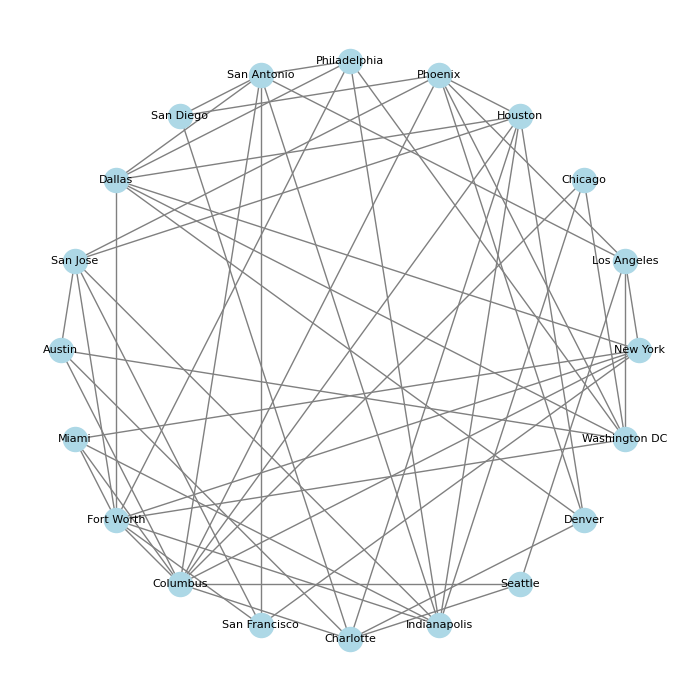
\includegraphics[width=2.5in]{plot_bfs.png}
\caption{Input graph for Breadth First Search (BFS)}
\label{fig_1}
\end{figure}

\subsection{Example}

\begin{figure}[!t]
\centering
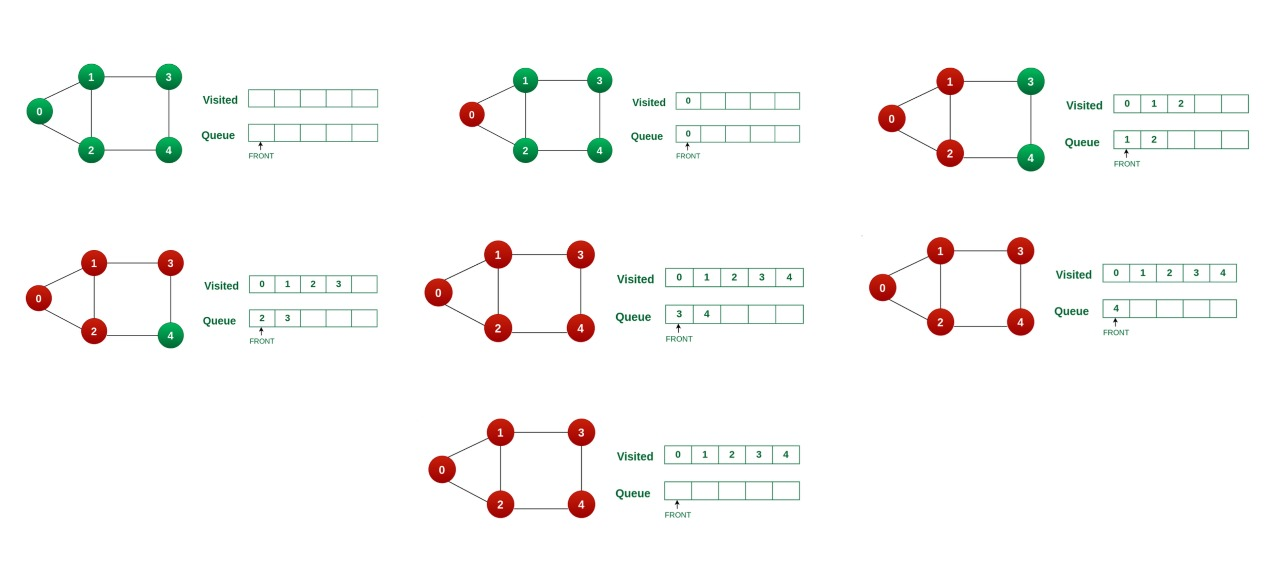
\includegraphics[width=2.5in]{EX_BFS.jpeg}
\caption{Manually solved example on Breadth First Search (BFS) \cite{bfs_gfg}}
\label{fig_2}
\end{figure}

We have an input graph and steps to solve the breadth first search an example manually. Below are the steps on solving the example in Fig. 2.

\begin{itemize}
    \item {\textbf{Step1:} Initially queue and visited arrays are empty.}
    \item {\textbf{Step2:} Push node 0 into queue and mark it visited.}
    \item {\textbf{Step3:} Remove node 0 from the front of queue and visit the unvisited neighbours and push them into queue.}
    \item {\textbf{Step4:} Remove node 1 from the front of queue and visit the unvisited neighbours and push them into queue.}
    \item {\textbf{Step5:} Remove node 2 from the front of queue and visit the unvisited neighbours and push them into queue.}
    \item {\textbf{Step6:} Remove node 3 from the front of queue and visit the unvisited neighbours and push them into queue. 
    
    As we can see that every neighbours of node 3 is visited, so move to the next node that are in the front of the queue.}
    \item {\textbf{Step7:} Remove node 4 from the front of queue and visit the unvisited neighbours and push them into queue. 
    
    As we can see that every neighbours of node 4 are visited, so move to the next node that is in the front of the queue.}
    
\end{itemize}

Using the same algorithm for input in Fig. 1 and example in Fig. 2. \cite{bfs_gfg}

\subsection{Algorithm}

\begin{algorithm}[H]
\caption{Breadth-First Search (BFS)}\label{alg:bfs}
\begin{algorithmic}
\Procedure{BFS}{$G, s$}
    \For{\textbf{each} vertex $u \in G.V - \{s\}$}
        \State $u.color \gets \text{WHITE}$
        \State $u.d \gets \infty$
        \State $u.\pi \gets \text{NIL}$
    \EndFor
    \State $s.color \gets \text{GRAY}$
    \State $s.d \gets 0$
    \State $s.\pi \gets \text{NIL}$
    \State $Q \gets$ empty queue
    \State \Call{Enqueue}{$Q, s$}
    \While{$Q \neq$ empty}
        \State $u \gets$ \Call{Dequeue}{$Q$}
        \For{\textbf{each} $v \in G.Adj[u]$}
            \If{$v.color == \text{WHITE}$}
                \State $v.color \gets \text{GRAY}$
                \State $v.d \gets u.d + 1$
                \State $v.\pi \gets u$
                \State \Call{Enqueue}{$Q, v$}
            \EndIf
        \EndFor
        \State $u.color \gets \text{BLACK}$
    \EndWhile
\EndProcedure
\end{algorithmic}
\end{algorithm}


\begin{lstlisting}[caption={Breadth-First Search Algorithm}]
import numpy as np
import networkx as nx
from collections import defaultdict
import matplotlib.pyplot as plt

cities = ["New York", "Los Angeles", "Chicago", "Houston", "Phoenix","Philadelphia", "San Antonio", "San Diego", "Dallas", "San Jose", "Austin", "Miami", "Fort Worth", "Columbus", "San Francisco", "Charlotte", "Indianapolis", "Seattle", "Denver", "Washington DC"]

# Creating new undirected graph for BFS
G_bfs = nx.Graph()
G_bfs.add_nodes_from(cities)

np.random.seed(0)

# Randomly connecting the cities for BFS
for city in cities:
    connections = np.random.choice(cities, size=np.random.randint(1, 6), replace=False)
    for conn in connections:
        if city != conn:
            G_bfs.add_edge(city, conn)

#Checking out the input
print("Nodes and Edges in the Graph:")
for node in G_bfs.nodes():
    edge_list = [f"({node}, {neighbor})" for neighbor in G_bfs.neighbors(node)]
    print(f"Node {node} is connected to:")
    for edge in edge_list:
        print(edge)

# Plotting the BFS graph
plt.figure(figsize=(7, 7))
nx.draw_circular(G_bfs, with_labels=True, node_color='lightblue', edge_color='gray', font_size=8)
plt.title("Input Graph of 20 USA Cities for BFS")

plt.savefig('/content/drive/My Drive/plot_bfs.png')
plt.show()

#Function Definition for BFS
def bfs(graph, start):
    visited = {key: False for key in cities}
    queue = []
    result = []

    queue.append(start)
    visited[start] = True

    while queue:
        node = queue.pop(0)
        result.append(node)

        for neighbor in graph[node]:
            if not visited[neighbor]:
                queue.append(neighbor) # appending nodes from left to right
                visited[neighbor] = True

    return result

start_node = "Miami"
print(G_bfs)
bfs_result = bfs(G_bfs, start_node)
print("Breadth-First Traversal (starting from {})".format(start_node))
print(bfs_result)

# Creating a directed graph to represent the BFS result
bfs_visual = nx.DiGraph()

# Adding edges based on the BFS traversal order
for i in range(len(bfs_result) - 1):

    bfs_visual.add_edge(bfs_result[i], bfs_result[i + 1])

# Plotting the graph
plt.figure(figsize=(7, 7))
pos = nx.circular_layout(bfs_visual)
nx.draw(bfs_visual, pos, with_labels=True, node_size=3000, node_color="skyblue", arrows=True)
plt.title("Visualization of BFS Traversal Order")

plt.savefig('/content/drive/My Drive/bfs_output.png')
plt.show()

\end{lstlisting}


\subsection{Implementation and Output}

\begin{figure}[!t]
\centering
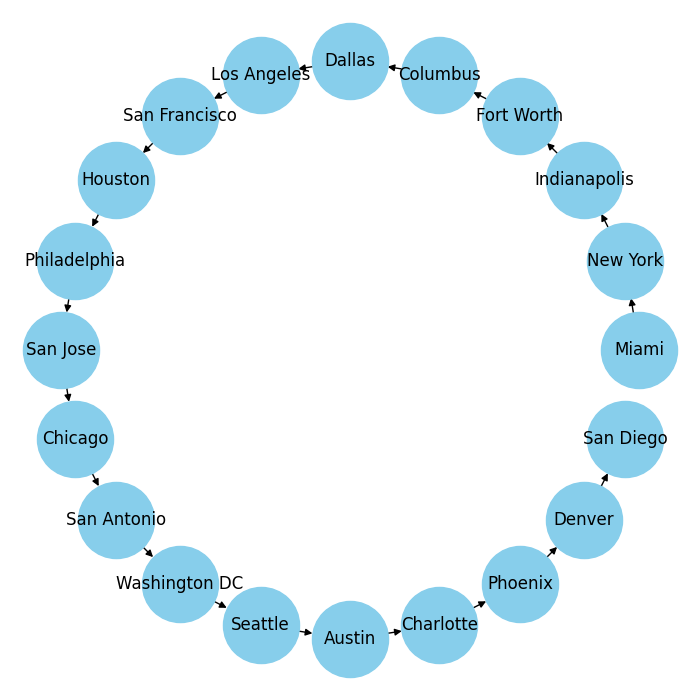
\includegraphics[width=2.5in]{bfs_output.png}
\caption{Output graph for Breadth First Search (BFS)}
\label{fig_3}
\end{figure}

Listing 1 shows that the algorithm is being implemented using python. Twenty major U.S. cities are used as input. There is a graphical representation of the input in Fig. 1. The function '\(bfs()\)' which has the input graph \(G\) and source vertex \(s\) as their parameters, is where the actual algorithm is being implemented. 

Our main assumption while implementing this algorithm is that the vertices are being added from left to right to the queue while traversing the graph. The variable \(result\) returns the list of cities in the order of traversal.

Fig. 3 gives the graphical representation of the traversal from the source vertex '\(Miami\)'.




\section{Bellman Ford Algorithm}

\subsection{Overview}

The Bellman-Ford algorithm operates on an input graph, \(G\), with ∣\(V\)∣ vertices and ∣\(E\)∣ edges. A single source vertex, \(s\), must be provided as well, as the Bellman-Ford algorithm is a single-source shortest path algorithm. No destination vertex needs to be supplied, however, because Bellman-Ford calculates the shortest distance to all vertices in the graph from the source vertex.

The Bellman-Ford algorithm, like Dijkstra's algorithm, uses the principle of relaxation to find increasingly accurate path length. Bellman-Ford, though, tackles two main issues with this process:

\begin{enumerate}
\item{If there are negative weight cycles, the search for a shortest path will go on forever.}
\item{Choosing a bad ordering for relaxations leads to exponential relaxations.}
\end{enumerate}{}{}

The detection of negative cycles is important, but the main contribution of this algorithm is in its ordering of relaxations. Dijkstra's algorithm is a greedy algorithm that selects the nearest vertex that has not been processed. Bellman-Ford, on the other hand, relaxes all of the edges.

Bellman-Ford labels the edges for a graph \(G\) as

\begin{equation}
\label{deqn_ex1}
\( e_1, e_2, \ldots, e_m \)
\end{equation}

and that set of edges is relaxed exactly \(V\) times, where \(V\) is the number of vertices in the graph.

Time Complexity: \(O(E*V)\), where \(V\) is the number of nodes and \(E\) is the number of edges.
Auxiliary Space: \(O(V)\). \cite{bellmanford_brilliant}

\begin{figure}[!t]
\centering
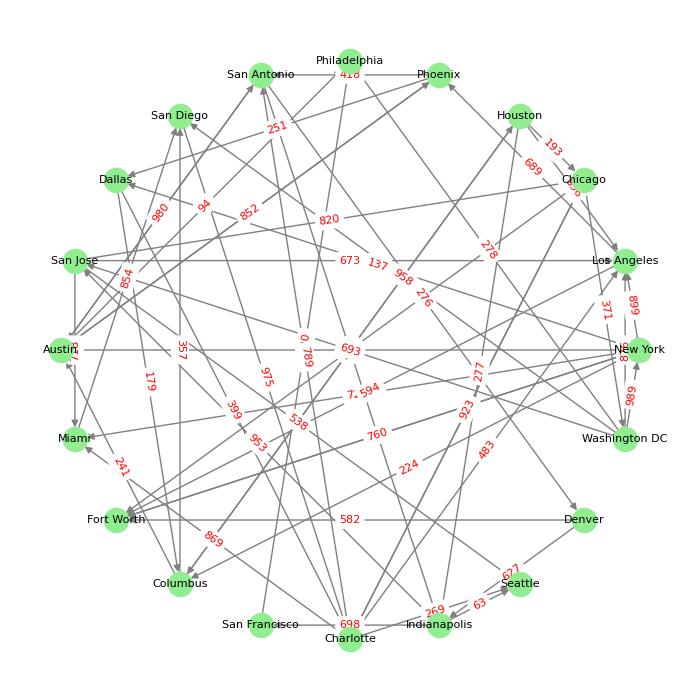
\includegraphics[width=2.5in]{plot_bf.png}
\caption{Input graph for Bellman Ford Algorithm}
\label{fig_3}
\end{figure}

\subsection{Problem Statement}
Implement a network between cities and connect them with random distance using graph data structure where vertices represent major cities of U.S. and edges represent the one-way connection between two cities and develop Bellman Ford algorithm to give the shortest path between source vertex and every other vertex.

\subsection{Input}
Fig. 4 shows the input graph created using networkx to solve single source shortest path problem using Bellman-Ford algorithm. The input graph \(G\) has 20 vertices and 52 edges. All the edges are directed and weighted in nature. The vertices represent the major cities of U.S. and the directed edges are randomly assigned in the graph, even the weights of the graph are randomly chosen and are not a reflection of real world. 

\subsection{Example}

\begin{figure}[!t]
\centering
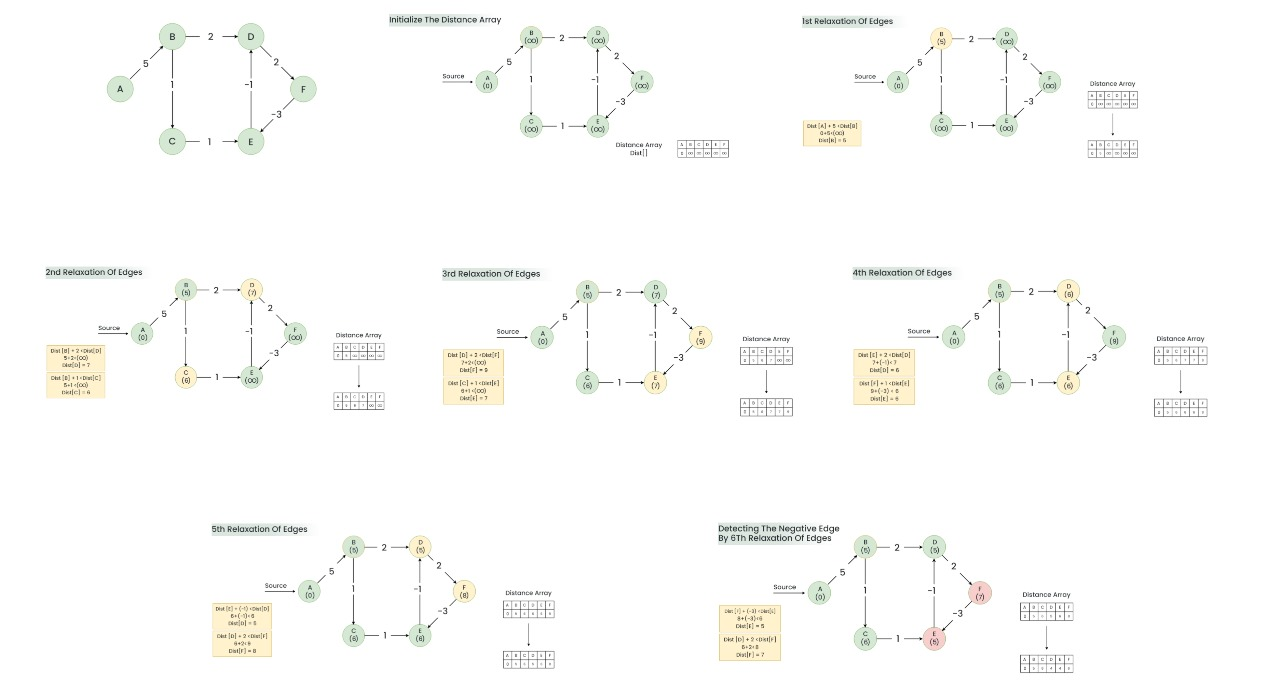
\includegraphics[width=2.5in]{EX_bellman-ford.jpeg}
\caption{Manually solved example on Bellman-Ford \cite{bellmanford_gfg}}
\label{fig_4}
\end{figure}

We have an example graph in Fig. 5


\begin{itemize}
    \item {\textbf{Step 1:} Initialize a distance array Dist[] to store the shortest distance for each vertex from the source vertex. Initially distance of source will be 0 and Distance of other vertices will be INFINITY.}

    
    \item {\textbf{Step 2:} Start relaxing the edges, during 1st Relaxation: 
    \begin{itemize}
        \item {Current Distance of B \(>\) (Distance of A) + (Weight of A to B) i.e. Infinity \(>\) 0 + 5}
        \item {Therefore, Dist[B] = 5}
    \end{itemize}
    }
    \item {\textbf{Step 3:} During 2nd Relaxation:}
    \begin{itemize}
        \item {Current Distance of D \(>\) (Distance of B) + (Weight of B to D) i.e. Infinity \(>\) 5 + 2. Hence, Dist[D] = 7.}
        \item {Current Distance of C \(>\) (Distance of B) + (Weight of B to C) i.e. Infinity \(>\) 5 + 1, Hence, Dist[C] = 6.}
    \end{itemize}
    \item {\textbf{Step 4:} During 3rd Relaxation:}
    \begin{itemize}
        \item {Current Distance of F \(>\) (Distance of D ) + (Weight of D to F) i.e. Infinity \(>\) 7 + 2. Hence, Dist[F] = 9.}
        \item {Current Distance of E \(>\) (Distance of C ) + (Weight of C to E) i.e. Infinity \(>\) 6 + 1. Hence, Dist[E] = 7.}
    \end{itemize}

    \item {\textbf{Step 5:} During 4th Relaxation:}
    \begin{itemize}
        \item {Current Distance of D \(>\) (Distance of E) + (Weight of E to D) i.e. 7 \(>\) 7 + (-1). Hence, Dist[D] = 6.}
        \item {Current Distance of E \(>\) (Distance of F ) + (Weight of F to E) i.e. 7 \(>\) 9 + (-3). Hence, Dist[E] = 6.}
    \end{itemize}

    \item {\textbf{Step 6:} During 5th Relaxation:}
    \begin{itemize}
        \item {Current Distance of F \(>\) (Distance of D) + (Weight of D to F) i.e. 9 \(>\) 6 + 2. Hence, Dist[F] = 8.}
        \item {Current Distance of D \(>\) (Distance of E ) + (Weight of E to D) i.e. 6 \(>\) 6 + (-1). Hence, Dist[E] = 5.}
        \item {Since the graph h 6 vertices, So during the 5th relaxation the shortest distance for all the vertices should have been calculated.}
    \end{itemize}

    \item {\textbf{Step 7:} Now the final relaxation i.e. the 6th relaxation should indicate the presence of negative cycle if there is any changes in the distance array of 5th relaxation.

    During the 6th relaxation, following changes can be seen:
    }
    \begin{itemize}
        \item {Current Distance of E \(>\) (Distance of F) + (Weight of F to E) i.e. 6 \(>\) 8 + (-3). Hence, Dist[E] = 5.}
        \item {Current Distance of F \(>\) (Distance of D ) + (Weight of D to F) i.e. 8 \(>\) 5 + 2. Hence, Dist[F] = 7.}
        \item {Since the graph h 6 vertices, So during the 5th relaxation the shortest distance for all the vertices should have been calculated.}
    \end{itemize}
    
\end{itemize}

Based on the previous steps, we know that there exists a negative cycle \( (D-> F-> E) \) \cite{bellmanford_gfg}.

\subsection{Algorithm}

\begin{algorithm}
\caption{Bellman-Ford Algorithm}\label{alg:bellman-ford}
\begin{algorithmic}
\Procedure{Bellman-Ford}{$G, w, s$}
\State \textsc{Initialize-Single-Source}$(G,s)$
\For{$i = 1$ \textbf{to} $|G.V| - 1$}
    \For{\textbf{each} edge $(u, v) \in G.E$}
        \State \textsc{Relax}$(u, v, w)$
    \EndFor
\EndFor
\For{\textbf{each} edge $(u, v) \in G.E$}
    \If{$v.d > u.d + w(u, v)$}
        \State \Return \textbf{false}
    \EndIf
\EndFor
\State \Return \textbf{true}
\EndProcedure
\Statex
\Procedure{Relax}{$u, v, w$}
    \If{$v.d > u.d + w(u, v)$}
        \State $v.d = u.d + w(u, v)$
        \State $v.\pi = u$
    \EndIf
\EndProcedure
\end{algorithmic}
\end{algorithm}


\begin{lstlisting}[caption={Bellman-Ford Algorithm}]
import numpy as np
import networkx as nx
from collections import defaultdict
import matplotlib.pyplot as plt

cities = ["New York", "Los Angeles", "Chicago", "Houston", "Phoenix","Philadelphia", "San Antonio", "San Diego", "Dallas", "San Jose", "Austin", "Miami", "Fort Worth", "Columbus", "San Francisco", "Charlotte", "Indianapolis", "Seattle", "Denver", "Washington DC"]

# Creating a new directed graph for Bellman-Ford
G_bf = nx.DiGraph()
G_bf.add_nodes_from(cities)

# Creating same graph every time the code is run
np.random.seed(0)

# Randomly assigning distances and connecting cities
for city in cities:
    connections = np.random.choice(cities, size=np.random.randint(1, 6), replace=False)
    for conn in connections:
        if city != conn:
            distance = np.random.randint(50, 1000)  # Random distance between 50 and 1000 miles
            G_bf.add_edge(city, conn, weight=distance)

count = 0

# Print the edges and their attributes (weights in this case)
print("\nEdges and their respective weights:")

for edge in G_bf.edges(data=True):
    source, target, attributes = edge
    weight = attributes['weight']
    print(f"Edge: {source} -> {target}, Weight: {weight}")
    count += 1

print(f'There are {count} number of edges in the graph')

# Plotting the Bellman-Ford graph with distances
plt.figure(figsize=(7, 7))

pos = nx.circular_layout(G_bf)
nx.draw_circular(G_bf, with_labels=True, node_color='lightgreen', edge_color='gray', font_size=8)
edge_labels = nx.get_edge_attributes(G_bf, 'weight')
nx.draw_networkx_edge_labels(G_bf, pos, edge_labels=edge_labels, font_color='red', font_size=8)

plt.title("Input Graph with Hypothetical Distances of 20 USA Cities for Bellman-Ford")
plt.savefig('/content/drive/My Drive/plot_bf.png')
plt.show()

def bellman_ford(graph, start):
    distance = {vertex: float('infinity') for vertex in graph}
    predecessor = {vertex: None for vertex in graph}

    distance[start] = 0

    for _ in range(len(graph) - 1):
        for node in graph:
            for neighbour, weight in graph[node].items():
                if distance[neighbour] > distance[node] + weight['weight']:
                    distance[neighbour] = distance[node] + weight['weight']
                    predecessor[neighbour] = node

    # Check for negative weight cycles
    for node in graph:
        for neighbour, weight in graph[node].items():
            if distance[neighbour] > distance[node] + weight['weight']:
                return "Negative weight cycle detected"

    return distance, predecessor

source_vertex = "Miami"
bf_distances, bf_predecessors = bellman_ford(G_bf, source_vertex)
for key, value in bf_distances.items():
  if value != 0:
    print(f"Bellman-Ford distance from {source_vertex} to {key} is {value} miles")

pos = nx.kamada_kawai_layout(G_bf)
plt.figure(figsize=(15, 10))  #Big size than rest of the graphs for better visibility

nx.draw_networkx_nodes(G_bf, pos, nodelist=[n for n in cities], node_color='lightgreen', node_size=700)
nx.draw_networkx_edges(G_bf, pos, edgelist=G_bf.edges(), edge_color='gray', width=2)
nx.draw_networkx_labels(G_bf, pos, font_size=12, font_weight='bold', font_family="sans-serif")
edge_labels = {(u, v): f"{d['weight']} mi" for u, v, d in G_bf.edges(data=True)}
nx.draw_networkx_edge_labels(G_bf, pos, edge_labels=edge_labels, font_color='red')

plt.title("Bellman-Ford distance from source vertex to all other vertices", fontsize=16)
plt.axis('off')
plt.savefig('/content/drive/My Drive/bf_output.png')
plt.show()

\end{lstlisting}

\subsection{Implementation and Output}

\begin{figure}[!t]
\centering
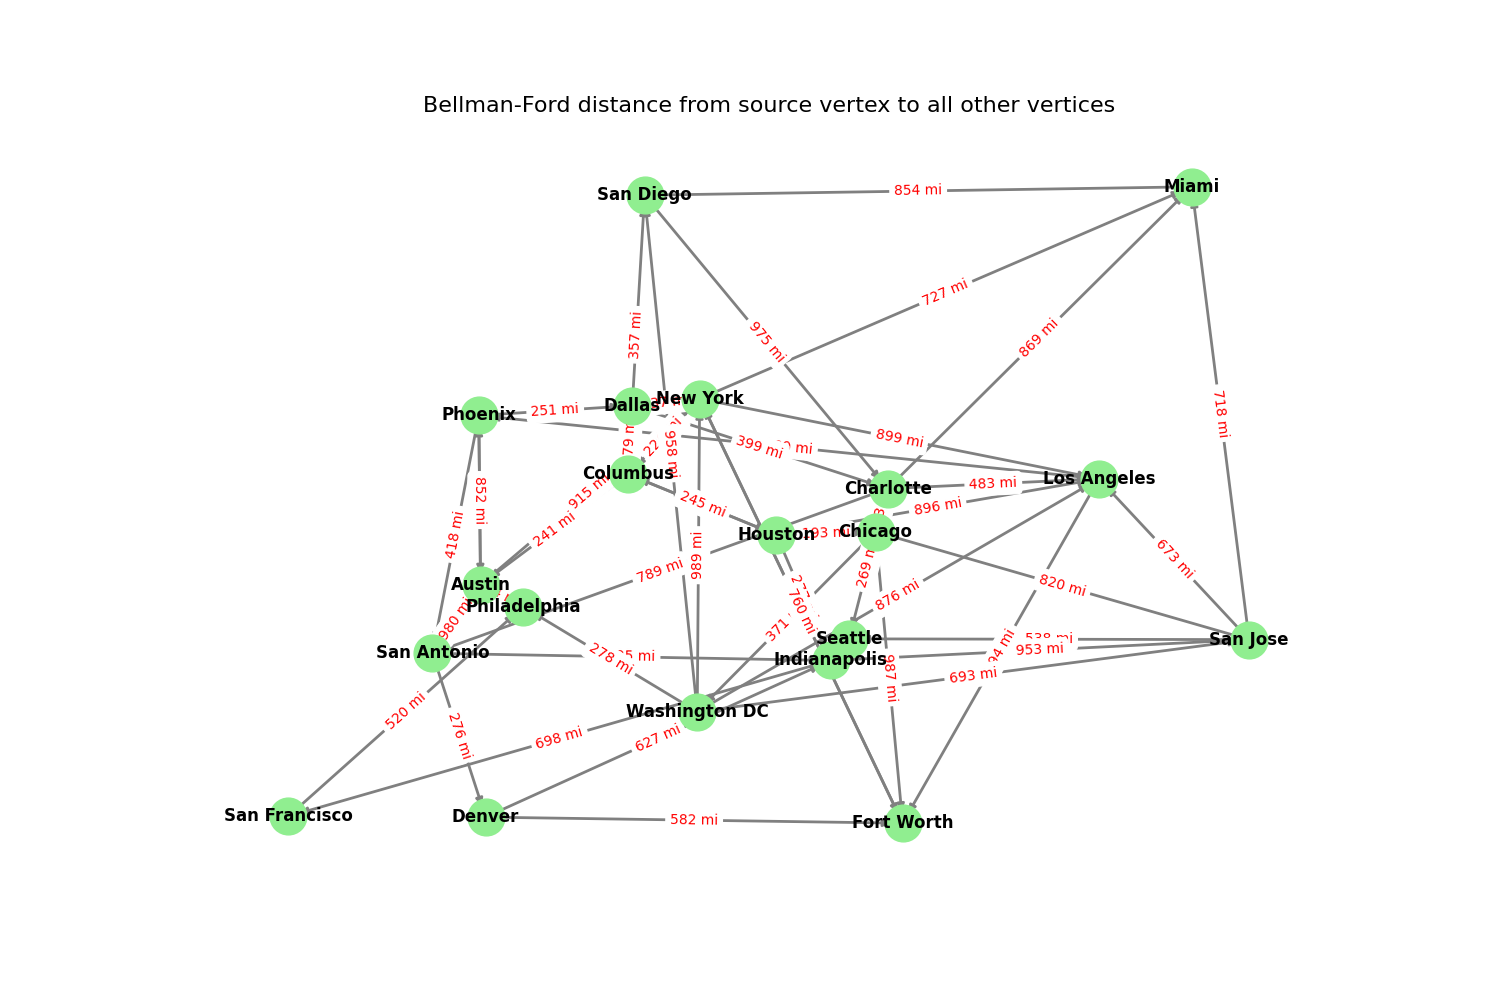
\includegraphics[width=2.5in]{bf_output.png}
\caption{Output graph for Bellman-Ford algorithm}
\label{fig_6}
\end{figure}

Listing 2 shows that bellman-ford algorithm is being implemented using python. Similar to breadth first search implementation, twenty major U.S. cities are used as input. It's graphical depiction can be seen in Fig. 4. The algorithm is being implemented in bellman-ford function definition with graph \(G\) and source vertex \(s\) as parameters.  It returns shortest distance between source vertex \(s\) and every other vertex \(v \in V\). 

The function also returns predecessors which would be helpful in finding new shorter distances from a similar vertex. Although it is not used while graphically plotting the output graph, you could see from the graph that some of the vertices are used as intermidiate vertices between multiple vertices more than once, which is where the predecessors dictionary was used. 

All the shortest distances are displayed and a graphical representation of the output is also given in Fig. 6.

\section{Conclusion}
In conclusion, the analysis of breadth first search and bellman-ford algorithms is helpful in building many applications. These algorithms provide lot of advantages to it's users. 

Some of it's applications and their advantages are :

\begin{itemize}
    \item {\textbf{Social Networking :} You can know the if a person is a first, second or third connection also known as degree of connection, by using BFS.} \cite{bfs_applications_gfg}
    \item {\textbf{Network Broadcasting :} This is another application of BFS, where packets in the network are brodcasted. An unique IP address is used when a broadcast message needs to be sent. It is very helpful when same message needs to be delivered across the network.} \cite{bfs_applications_gfg}
    \item {\textbf{GPS Navigation :} As suggested by the input in the report, this is definitely an important application for getting not only the neighbors of a particular city (BFS), but also the shortest path to every node given in the input graph (bellman-ford).} \cite{bfs_applications_gfg}
    \item {\textbf{Traffic Engineering :} Here, bellman-ford is being used and based on the traffic, it will provide optimal solutions based on metrics that can affect travel time.} \cite{ChatGPT}
    \item {\textbf{Network Routing :} Some distance vector routing protocols like Routing Information Protocol (RIP) and Border Gateway Protocol (BGP) use bellman-ford algorithm as, each node needs to update it's information based on the information recieved from previous nodes, which, in-turn will help in finding the shortest path from source to destination node.} \cite{ChatGPT}
\end{itemize}


\bibliographystyle{plain}
\bibliography{references}

\end{document}